%!TEX program = xelatex
\documentclass[cn,blue,14pt,normal]{elegantnote}

\title{西安单阈值控制响应图谱分析笔记}
\author{西安阈值控制分析笔记}
\institute{SIQR 模型与医疗阈值控制}
\version{0.1}
\date{\today}

\usepackage{amsmath,amssymb}
\usepackage{booktabs}
\usepackage{array}
\usepackage{graphicx}
\usepackage{float}
\usepackage{xurl}
\usepackage{hyperref}
\hypersetup{hidelinks}

\graphicspath{
  {../}
  {../eta_landscape/}
  {../representative_eta_panels/}
  {../cost_weight_analysis/}
  {../eta_c0_heatmap/}
  {../representative_c0_panels/}
  {../high_c0_stress_test_panels/}
}
\numberwithin{equation}{section}
\allowdisplaybreaks[3]
\renewcommand{\arraystretch}{1.12}

\newcommand{\Itcum}{I_{t_{\rm cum}}}
\newcommand{\Rzero}{R_0}
\newcommand{\Reff}{R_e}

\begin{document}

\maketitle

\section{问题与符号}

这份笔记整理西安疫情控制比较中的单阈值控制响应图谱。研究对象不是重新拟合数据，而是在已经校准好的 SIQR 模型下，观察情景一阈值控制在不同社区感染者阈值 $\eta$ 和常态接触水平 $c_0$ 下的数值表现。

模型变量沿用西安比较文档中的记号。$S(t)$ 表示社区易感者，$I(t)$ 表示社区感染者，$S_q(t)$ 表示隔离易感者，$I_q(t)$ 表示隔离感染者。每日新增社区感染者记为 $I_{\rm new}(t)$，每日新增隔离感染者记为 $I_{q_{\rm new}}(t)$。累计社区感染和累计隔离感染分别记为 $I_{\rm cum}(t)$ 和 $I_{q_{\rm cum}}(t)$，总累计感染定义为
\begin{equation}
  \Itcum(t)=I_{\rm cum}(t)+I_{q_{\rm cum}}(t).
\end{equation}

控制变量为接触率 $c(t)$ 和隔离率 $q(t)$。TDINN控制使用文献学习得到的时间函数 $c_{\rm TDINN}(t)$ 与 $q_{\rm TDINN}(t)$。常规控制取
\begin{equation}
  c(t)\equiv c_0,\qquad q(t)\equiv q_0=0.3230.
\end{equation}
在基准阈值图中取 $c_0=12.8872$。在 $c_0$ 敏感性图中，TDINN控制仍作为文献函数参照；情景一阈值控制和常规控制均使用当前给定的 $c_0$ 重新计算。

\begin{note}
  这里的 $\eta$ 是模型中的社区感染者阈值，不是 ICU 床位数本身。$\eta=100,520,1300$ 等取值在本笔记中只作为数学阈值或补充计算点使用。
\end{note}

\section{模型与开环阈值控制}

人口规模下的带隔离 SIQR 模型写为
\begin{align}
  \dot S
  &=
  -\frac{c(t)[\beta+q(t)(1-\beta)]S(t)I(t)}{N},\\
  \dot I
  &=
  \frac{\beta c(t)(1-q(t))S(t)I(t)}{N}-\gamma I(t),\\
  \dot S_q
  &=
  \frac{(1-\beta)c(t)q(t)S(t)I(t)}{N},\\
  \dot I_q
  &=
  \frac{\beta c(t)q(t)S(t)I(t)}{N}-\delta_q I_q(t).
\end{align}
累计变量满足
\begin{equation}
  \dot I_{\rm cum}
  =
  \frac{\beta c(t)(1-q(t))S(t)I(t)}{N},
  \qquad
  \dot I_{q_{\rm cum}}
  =
  \frac{\beta c(t)q(t)S(t)I(t)}{N}.
\end{equation}

西安参数固定为
\begin{equation}
  N=13{,}163{,}000,\qquad
  \beta=0.1498,\qquad
  \gamma=0.2953,\qquad
  \delta_q=0.3531.
\end{equation}
初值拟合只估计 $I_0$，并令 $S_0=N-I_0$。这个 $I_0$ 是模型校准种子，不应解释为现实中的整数病例数。

情景一阈值控制要求在控制期内维持
\begin{equation}
  I(t)=\eta.
\end{equation}
由 $\dot I=0$ 得到控制期隔离率
\begin{equation}
  q_c(t)
  =
  1-\frac{\gamma N}{\beta c_0 S_{\rm th}(t)}.
  \label{eq:q-control}
\end{equation}
其中
\begin{equation}
  S_{\rm th}(t)
  =
  \bar S+(S^*-\bar S)
  \exp\left[-\frac{c_0\eta(t-t_1)}{N}\right],
  \qquad
  \bar S=\frac{\gamma N(1-\beta)}{\beta c_0}.
  \label{eq:S-th}
\end{equation}
$S^*$ 是常规轨道首次达到 $I=\eta$ 时的易感者数量，$t_1$ 是控制启动时间。控制结束时间为
\begin{equation}
  t_2
  =
  t_1+
  \frac{N}{c_0\eta}
  \log\frac{S^*-\bar S}{S_c-\bar S},
  \qquad
  S_c=\frac{\gamma N}{\beta c_0(1-q_0)}.
  \label{eq:t2}
\end{equation}
因此控制时长为
\begin{equation}
  \Delta t=t_2-t_1.
\end{equation}

\begin{remark}
  式 \eqref{eq:q-control} 中的 $q_c(t)$ 是提前计算好的时间函数。数值模拟时只按照时间 $t$ 调用它，不根据实时积分得到的 $S(t)$ 临时调整隔离率。因此这里分析的是时间开环控制，不是状态反馈控制。
\end{remark}

\section{阈值 \texorpdfstring{$\eta$}{eta} 的影响}

图~\ref{fig:eta_landscape} 汇总了 $\eta\in[100,30000]$ 下的主要指标。数值上，所有扫描点都满足可行性状态 \texttt{ok}，平台期误差为 0。这说明在当前参数范围内，式 \eqref{eq:q-control} 给出的开环隔离率没有超过 $[0,1]$，并且能够在平台期保持 $I(t)=\eta$。

本节中的清零终止时刻记为 $t_{\rm end}$。计算时先在后期常规阶段的首次积分中由 $I(t_{\rm end})=1$ 解出 $S_{\rm end}$，再按主论文公式从 $S_c$ 积分到 $S_{\rm end}$ 得到 $t_{\rm end}-t_2$.

\begin{figure}[htbp]
  \centering
  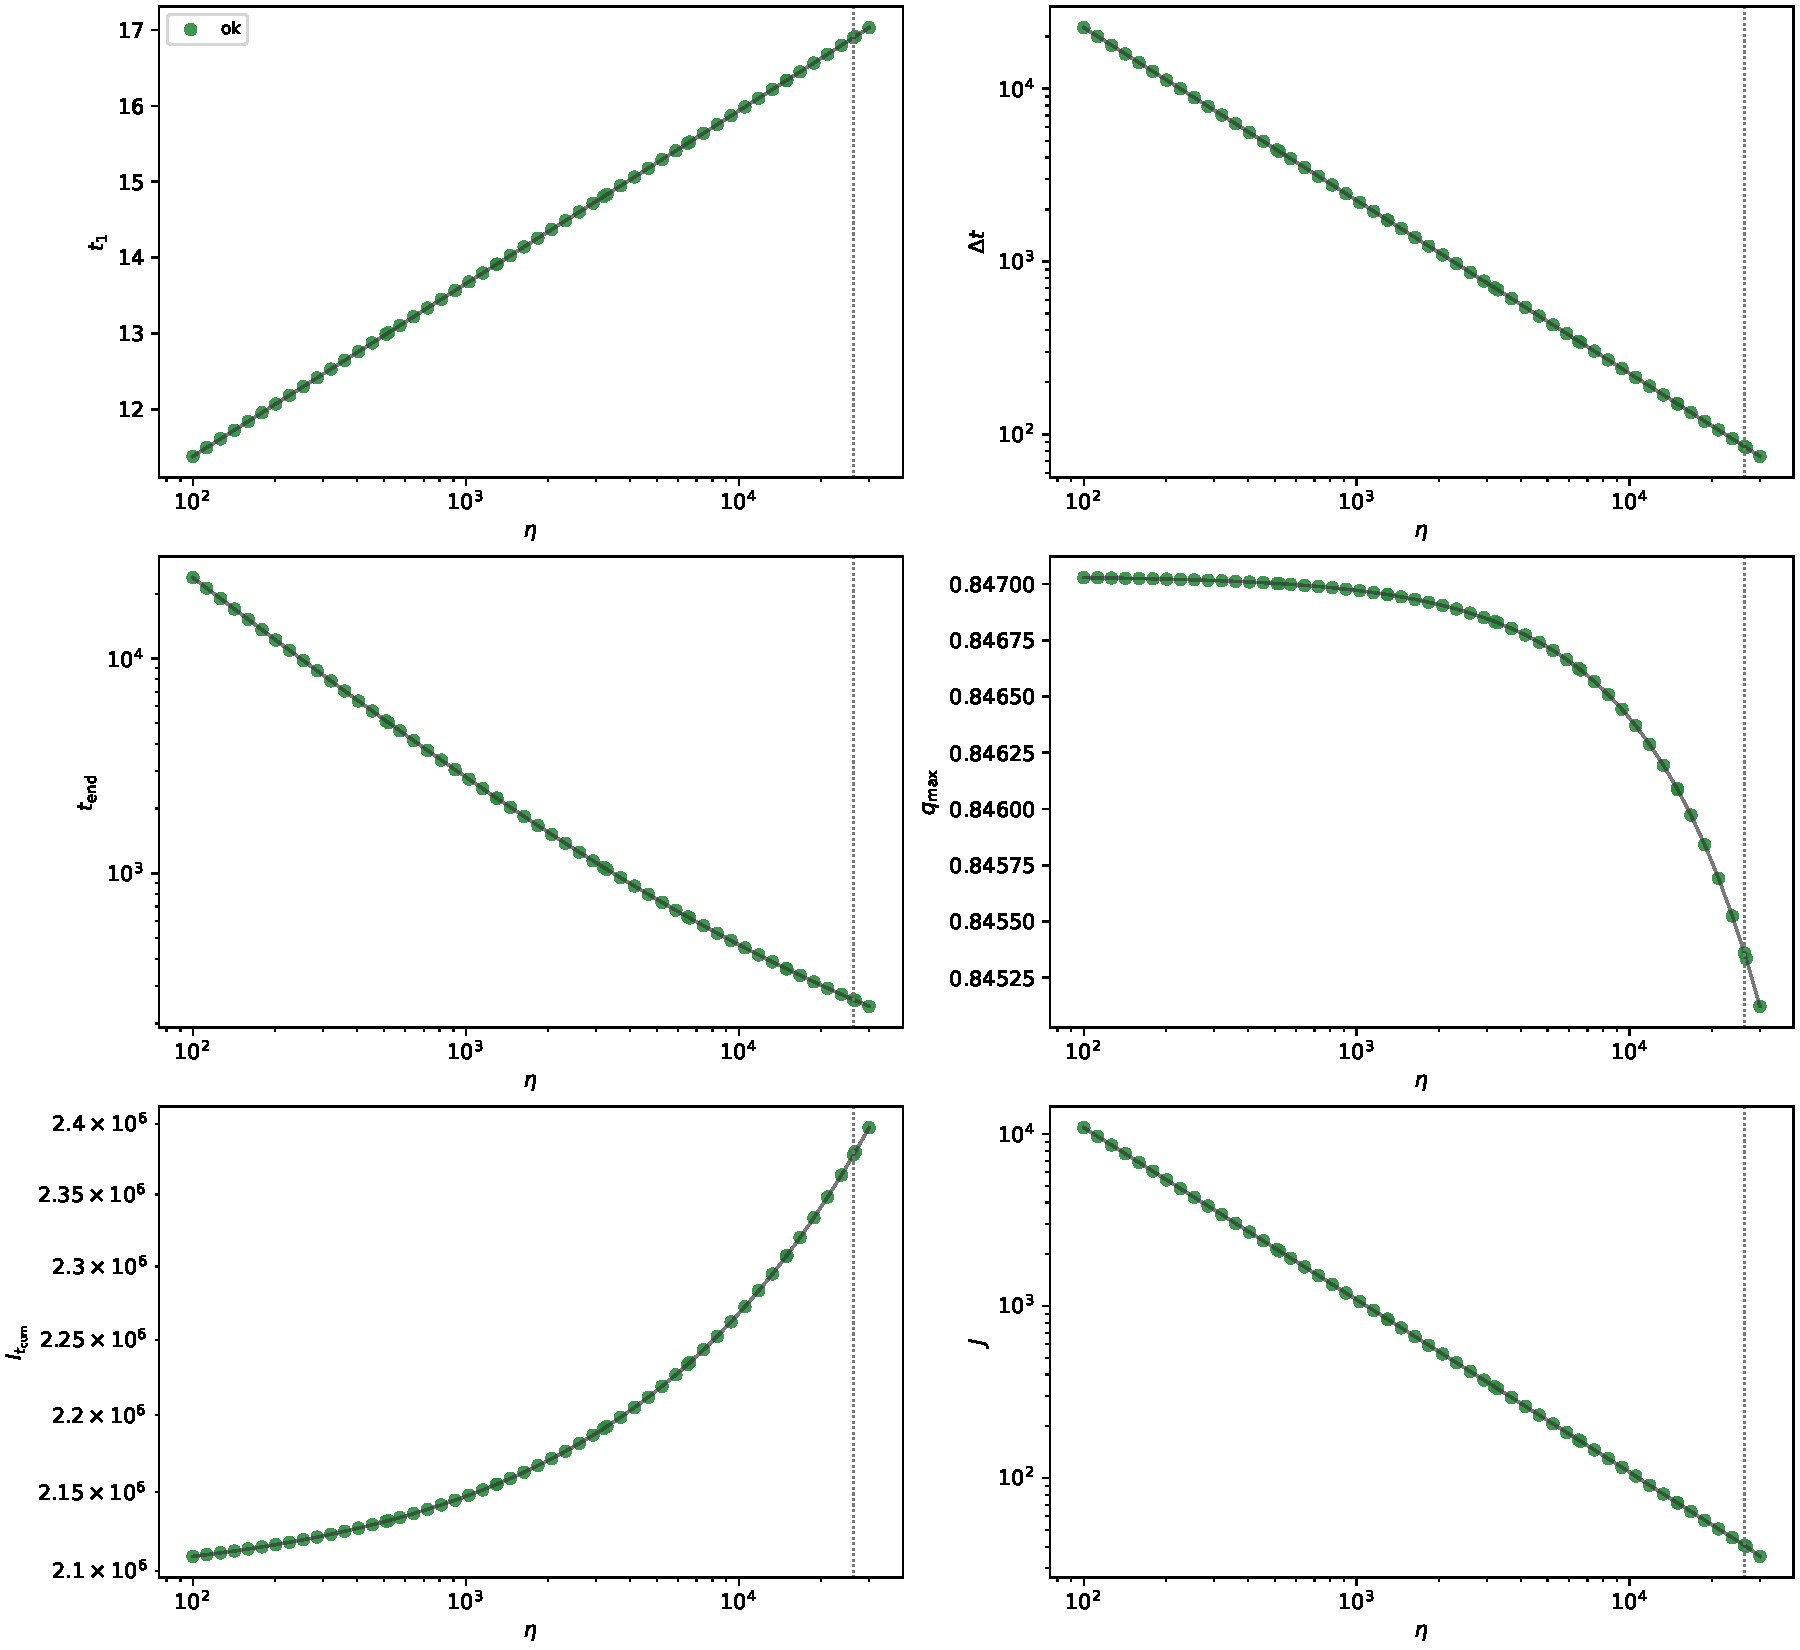
\includegraphics[width=0.95\textwidth,height=0.64\textheight,keepaspectratio]{eta_landscape_sensitivity.pdf}
  \caption{不同阈值 $\eta$ 下情景一阈值控制的响应图谱。横轴采用对数尺度。}
  \label{fig:eta_landscape}
\end{figure}

表~\ref{tab:eta-rep} 给出三个代表阈值的数值。固定 $c_0=12.8872$ 时，降低 $\eta$ 会提前启动控制，但更明显的变化出现在 $\Delta t$ 和 $t_{\rm end}$ 上。

\begin{table}[H]
  \centering
  \caption{$c_0=12.8872$ 下代表阈值的主要指标。}
  \label{tab:eta-rep}
  \resizebox{\textwidth}{!}{
  \begin{tabular}{cccccccc}
    \toprule
    $\eta$ & $t_1$ & $t_2$ & $\Delta t$ & $t_{\rm end}$ & $\Itcum$ & $q_{\max}$ & $J$\\
    \midrule
    100 & 11.38 & 22534.66 & 22523.29 & 23748.32 & $2.1093\times 10^6$ & 0.8470 & 5442.32\\
    1300 & 13.91 & 1746.03 & 1732.12 & 2233.26 & $2.1553\times 10^6$ & 0.8470 & 418.36\\
    26326 & 16.90 & 101.97 & 85.07 & 258.11 & $2.3779\times 10^6$ & 0.8454 & 20.36\\
    \bottomrule
  \end{tabular}}
\end{table}

这里的主要结构来自式 \eqref{eq:t2}。当 $\eta$ 变小，平台期内 $I(t)=\eta$ 也变小，易感者消耗速度随之降低；同时 $\Delta t$ 中有显式因子 $1/\eta$。因此，低阈值可以降低感染峰值，但会把控制期拉得很长。以 $\eta=100$ 为例，$\Delta t$ 达到 $22523.29$ 天，这更像一种长期低感染水平维持的数学情形，而不是短期控制后退出。

表中的 $q_{\max}$ 表示平台控制段所需隔离率的最大值。当前情景一公式下 $q_c(t)$ 随 $S_{\rm th}(t)$ 下降而下降，因此最大值在启动端点取得；但 $q_{\max}$ 是强度指标，$q_c(t)$ 是整条时间开环控制函数，二者不应混用。

图~\ref{fig:eta100-panel}--图~\ref{fig:eta26326-panel} 进一步给出低、中、高三个阈值下的轨迹。$\eta=100$ 时，社区感染者很早进入平台，但平台时间很长；$\eta=26326$ 时，平台时间明显缩短，但允许的感染峰值也更高。

\begin{figure}[htbp]
  \centering
  
\includegraphics[width=0.95\textwidth,height=0.64\textheight,keepaspectratio]{panels_eta100.pdf}
  \caption{$\eta=100$ 时的三类轨迹比较。该阈值用于观察低阈值长期平台现象。}
  \label{fig:eta100-panel}
\end{figure}

\begin{figure}[htbp]
  \centering
  
\includegraphics[width=0.95\textwidth,height=0.64\textheight,keepaspectratio]{panels_eta1300.pdf}
  \caption{$\eta=1300$ 时的三类轨迹比较。}
  \label{fig:eta1300-panel}
\end{figure}

\begin{figure}[htbp]
  \centering
  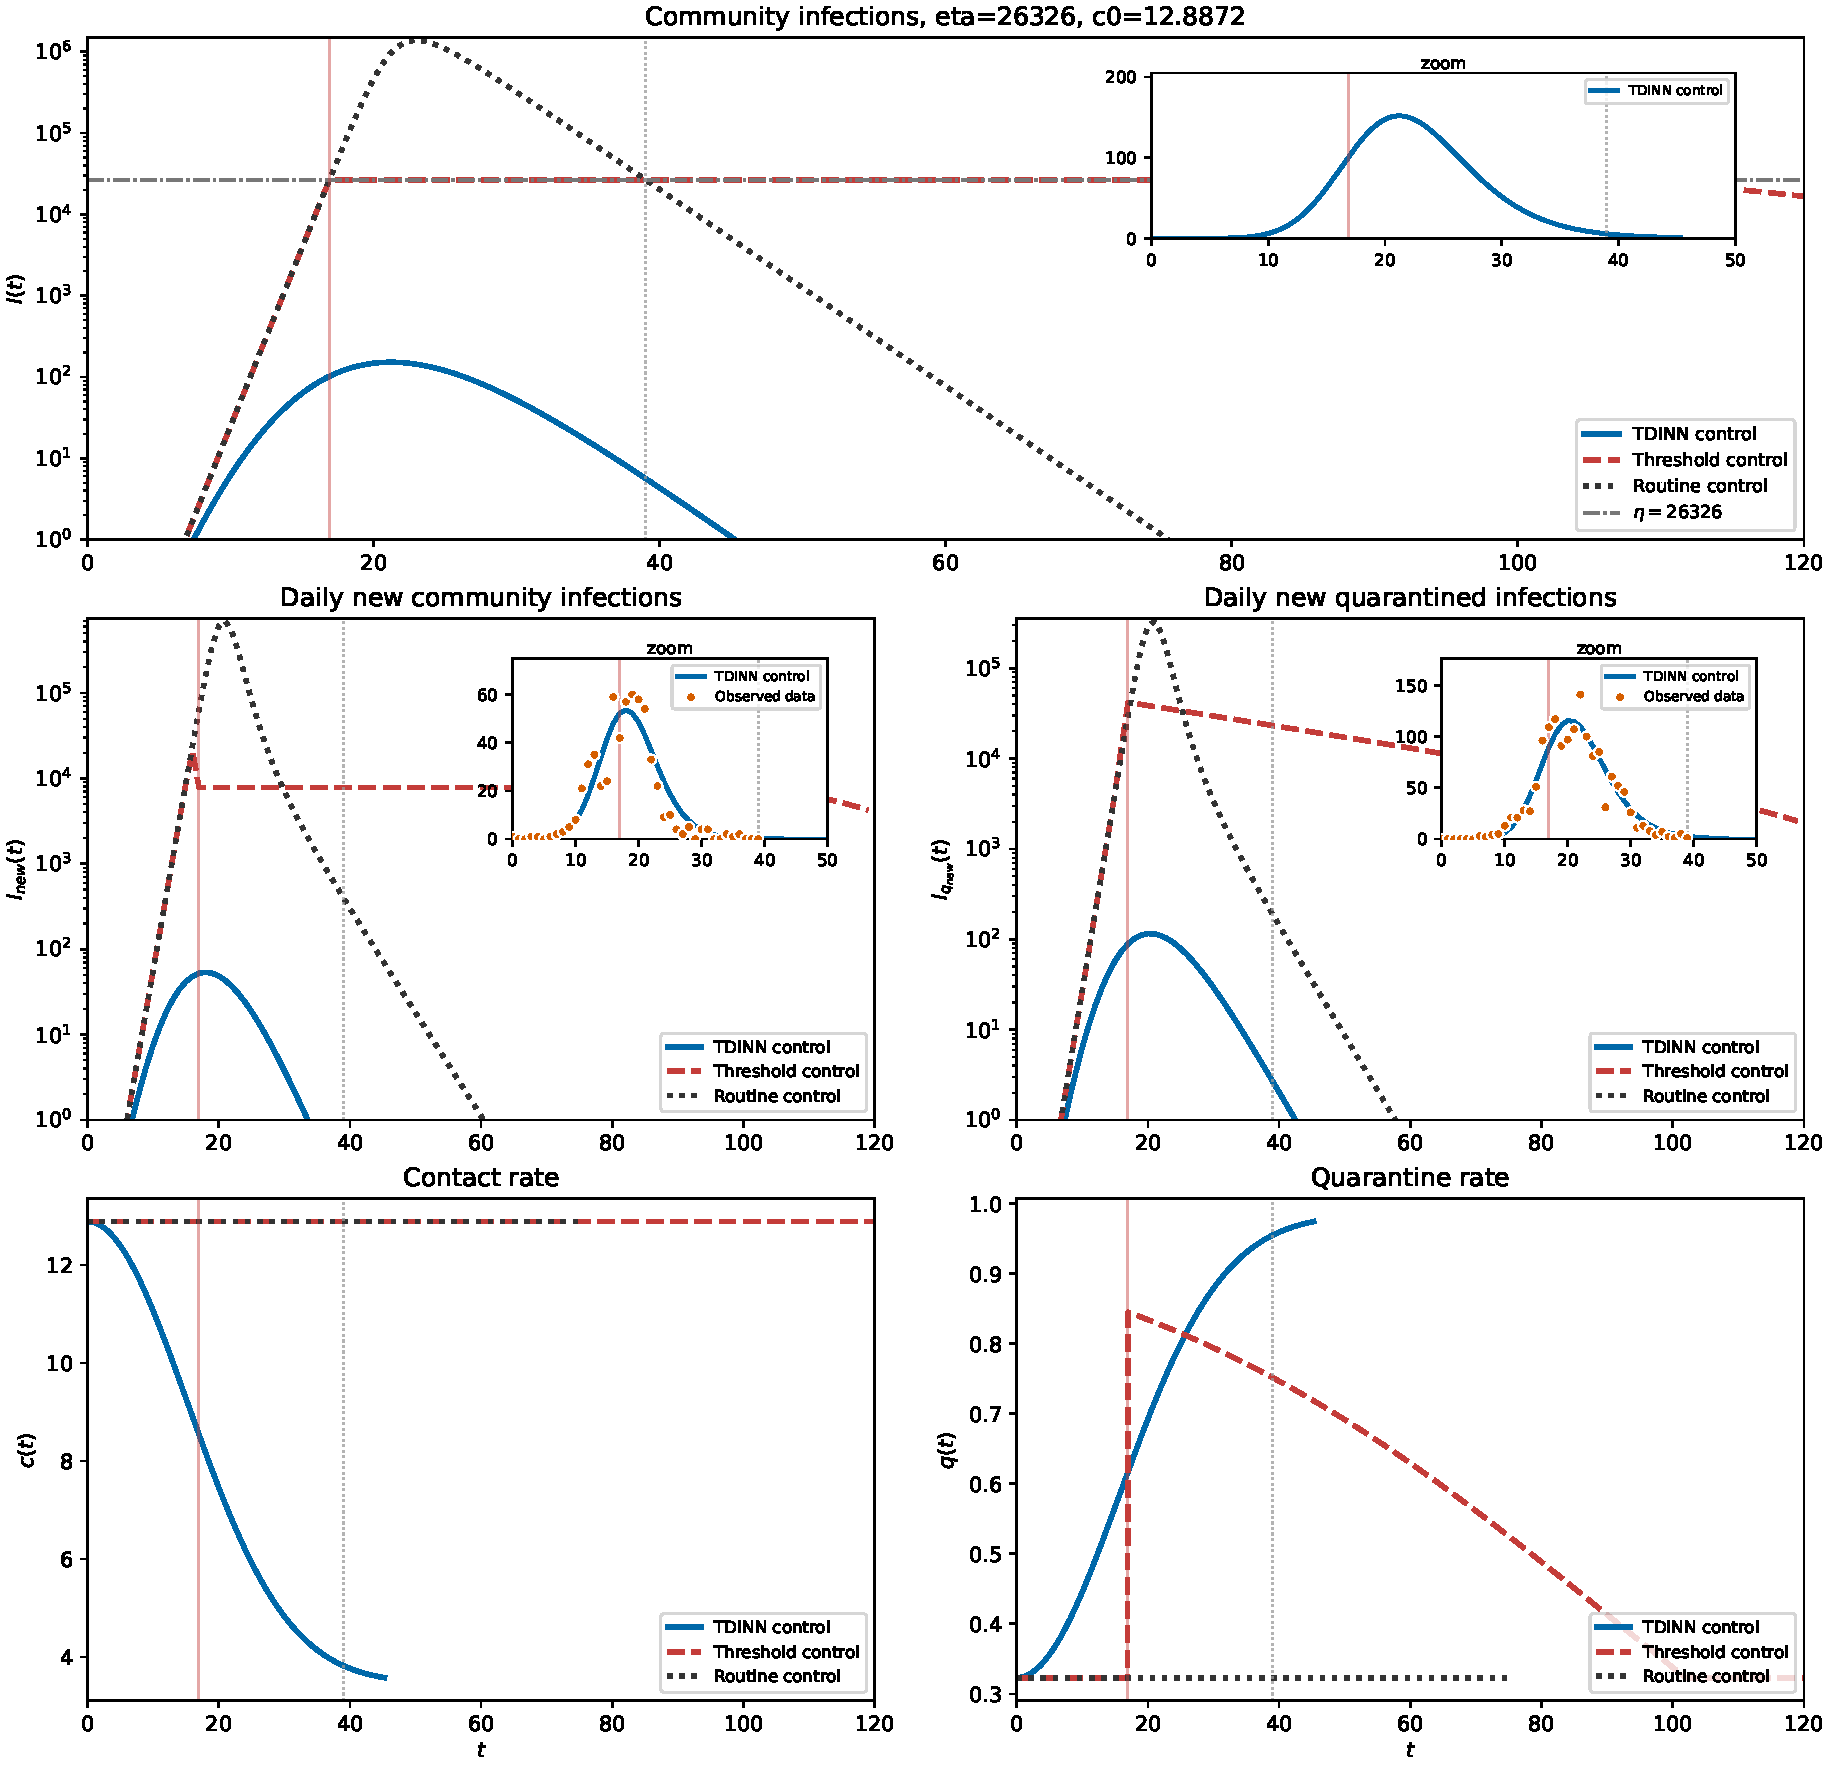
\includegraphics[width=0.95\textwidth,height=0.64\textheight,keepaspectratio]{panels_eta26326.pdf}
  \caption{$\eta=26326=0.002N$ 时的三类轨迹比较。}
  \label{fig:eta26326-panel}
\end{figure}

\section{控制成本}

本笔记使用二次加权总成本作为主要成本指标。单独的归一化分项成本为
\begin{equation}
  J_c=\int \frac{(c_0-c(t))_+}{c_0}\,dt,
\end{equation}
\begin{equation}
  J_q=\int \frac{(q(t)-q_0)_+}{1-q_0}\,dt.
\end{equation}
其中 $J_c$ 与 $J_q$ 只用于区分成本来源，不相加为综合指标。主要成本记为
\begin{equation}
  J
  =
  \int
  \left[
    w_c\left(\frac{(c_0-c(t))_+}{c_0}\right)^2
    +
    w_q\left(\frac{(q(t)-q_0)_+}{1-q_0}\right)^2
  \right]dt.
  \label{eq:Jcost}
\end{equation}
下文默认取 $w_c=1,w_q=2$。对于情景一阈值控制，控制期内 $c(t)\equiv c_0$，因此式 \eqref{eq:Jcost} 中接触率控制项为 0，主要变化来自隔离率项。

\begin{figure}[htbp]
  \centering
  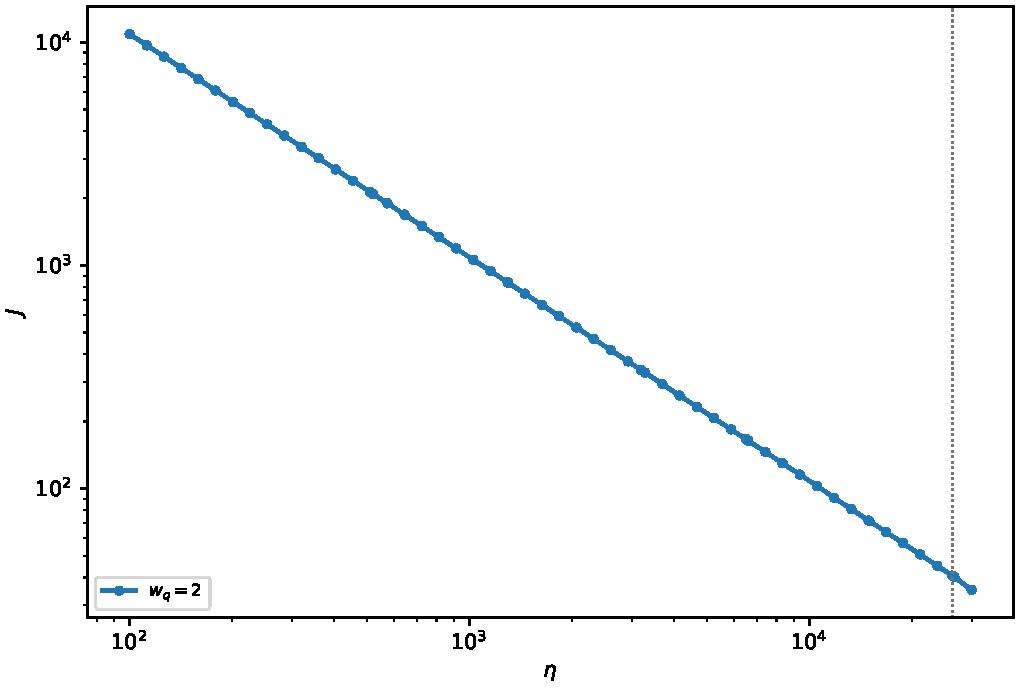
\includegraphics[width=0.82\textwidth,height=0.52\textheight,keepaspectratio]{cost_summary_wq2.pdf}
  \caption{固定 $w_c=1,w_q=2$ 时二次加权总成本 $J$ 随 $\eta$ 的变化。}
  \label{fig:cost-weight}
\end{figure}

从表~\ref{tab:eta-rep} 和图~\ref{fig:cost-weight} 可以看出，低阈值下总成本较高，主要不是因为每天的隔离率都非常接近 1，而是因为控制期 $\Delta t$ 很长。较高阈值下平台时间缩短，总成本随之降低，但这同时允许更高的社区感染者峰值。

\section{\texorpdfstring{$(\eta,c_0)$}{eta-c0} 二维敏感性}

主敏感性区间取
\begin{equation}
  c_0\in[6,13],
  \qquad
  \eta\in[100,30000].
\end{equation}
这里的 $c_0$ 表示常态接触水平。TDINN控制固定为文献函数参照；情景一阈值控制和常规控制均使用当前给定的 $c_0$ 重新计算。

\begin{figure}[htbp]
  \centering
  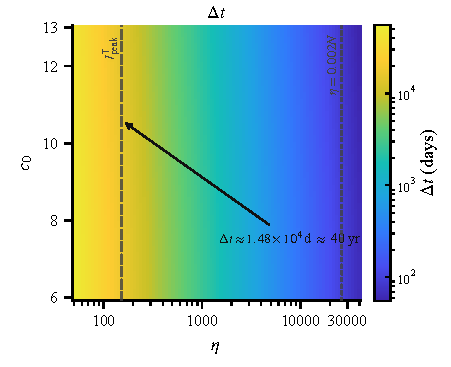
\includegraphics[width=0.95\textwidth,height=0.56\textheight,keepaspectratio]{heatmap_control_duration.pdf}
  \caption{$(\eta,c_0)$ 平面上的控制时长 $\Delta t$。}
  \label{fig:heat-duration}
\end{figure}

\begin{figure}[htbp]
  \centering
  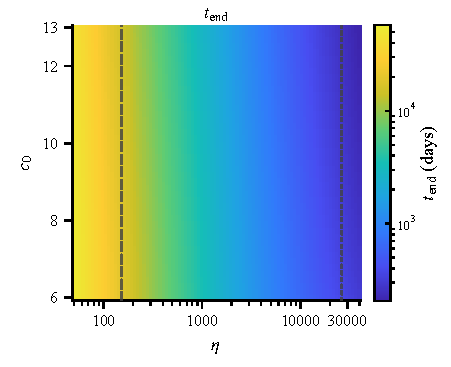
\includegraphics[width=0.95\textwidth,height=0.56\textheight,keepaspectratio]{heatmap_clear_time.pdf}
  \caption{$(\eta,c_0)$ 平面上的清零终止时刻 $t_{\rm end}$。}
  \label{fig:heat-clear}
\end{figure}

\begin{figure}[htbp]
  \centering
  
\includegraphics[width=0.95\textwidth,height=0.56\textheight,keepaspectratio]{heatmap_J.pdf}
  \caption{$(\eta,c_0)$ 平面上的二次加权总成本 $J$。}
  \label{fig:heat-J}
\end{figure}

表~\ref{tab:c0-rep} 选取 $c_0=6,12.8872,20$ 和三个代表阈值作对照。其中 $c_0=20$ 不属于主区间，只作为较高接触率补充计算。可以看到，随着 $c_0$ 增大，阈值更早被触及，因此 $t_1$ 明显提前；同时 $\Delta t$ 和 $t_{\rm end}$ 缩短。但是所需最大隔离率 $q_{\max}$ 增大。

\begin{table}[H]
  \centering
  \caption{不同 $c_0$ 与代表阈值下的数值指标。}
  \label{tab:c0-rep}
  \resizebox{\textwidth}{!}{
  \begin{tabular}{cccccccc}
    \toprule
    $c_0$ & $\eta$ & $t_1$ & $\Delta t$ & $t_{\rm end}$ & $\Itcum$ & $q_{\max}$ & $J$\\
    \midrule
    6 & 100 & 36.75 & 27474.82 & 29287.83 & $1.7304\times10^6$ & 0.6714 & 2558.35\\
    6 & 1300 & 44.94 & 2111.71 & 2866.86 & $1.7980\times10^6$ & 0.6712 & 196.33\\
    6 & 26326 & 54.65 & 102.45 & 379.97 & $2.1291\times10^6$ & 0.6660 & 9.18\\
    12.8872 & 100 & 11.38 & 22523.29 & 23748.32 & $2.1093\times10^6$ & 0.8470 & 5442.32\\
    12.8872 & 1300 & 13.91 & 1732.12 & 2233.26 & $2.1553\times10^6$ & 0.8470 & 418.36\\
    12.8872 & 26326 & 16.90 & 85.07 & 258.11 & $2.3779\times10^6$ & 0.8454 & 20.36\\
    20 & 100 & 6.64 & 17746.63 & 18728.53 & $2.1444\times10^6$ & 0.9014 & 5665.89\\
    20 & 1300 & 8.12 & 1364.88 & 1765.76 & $2.1812\times10^6$ & 0.9014 & 435.35\\
    20 & 26326 & 9.86 & 67.14 & 204.96 & $2.3589\times10^6$ & 0.9005 & 21.28\\
    \bottomrule
  \end{tabular}}
\end{table}

这说明 $c_0$ 的作用主要体现在两个方面。第一，较大的 $c_0$ 使常规阶段增长更快，阈值控制更早启动。第二，较大的 $c_0$ 需要更高的隔离率来满足 $\dot I=0$。在当前扫描中，$q_{\max}$ 没有超过 1，因此理论上仍可构造；但当 $c_0=20$ 时，$q_{\max}$ 已接近 0.90，实施含义需要另行讨论。

\begin{figure}[htbp]
  \centering
  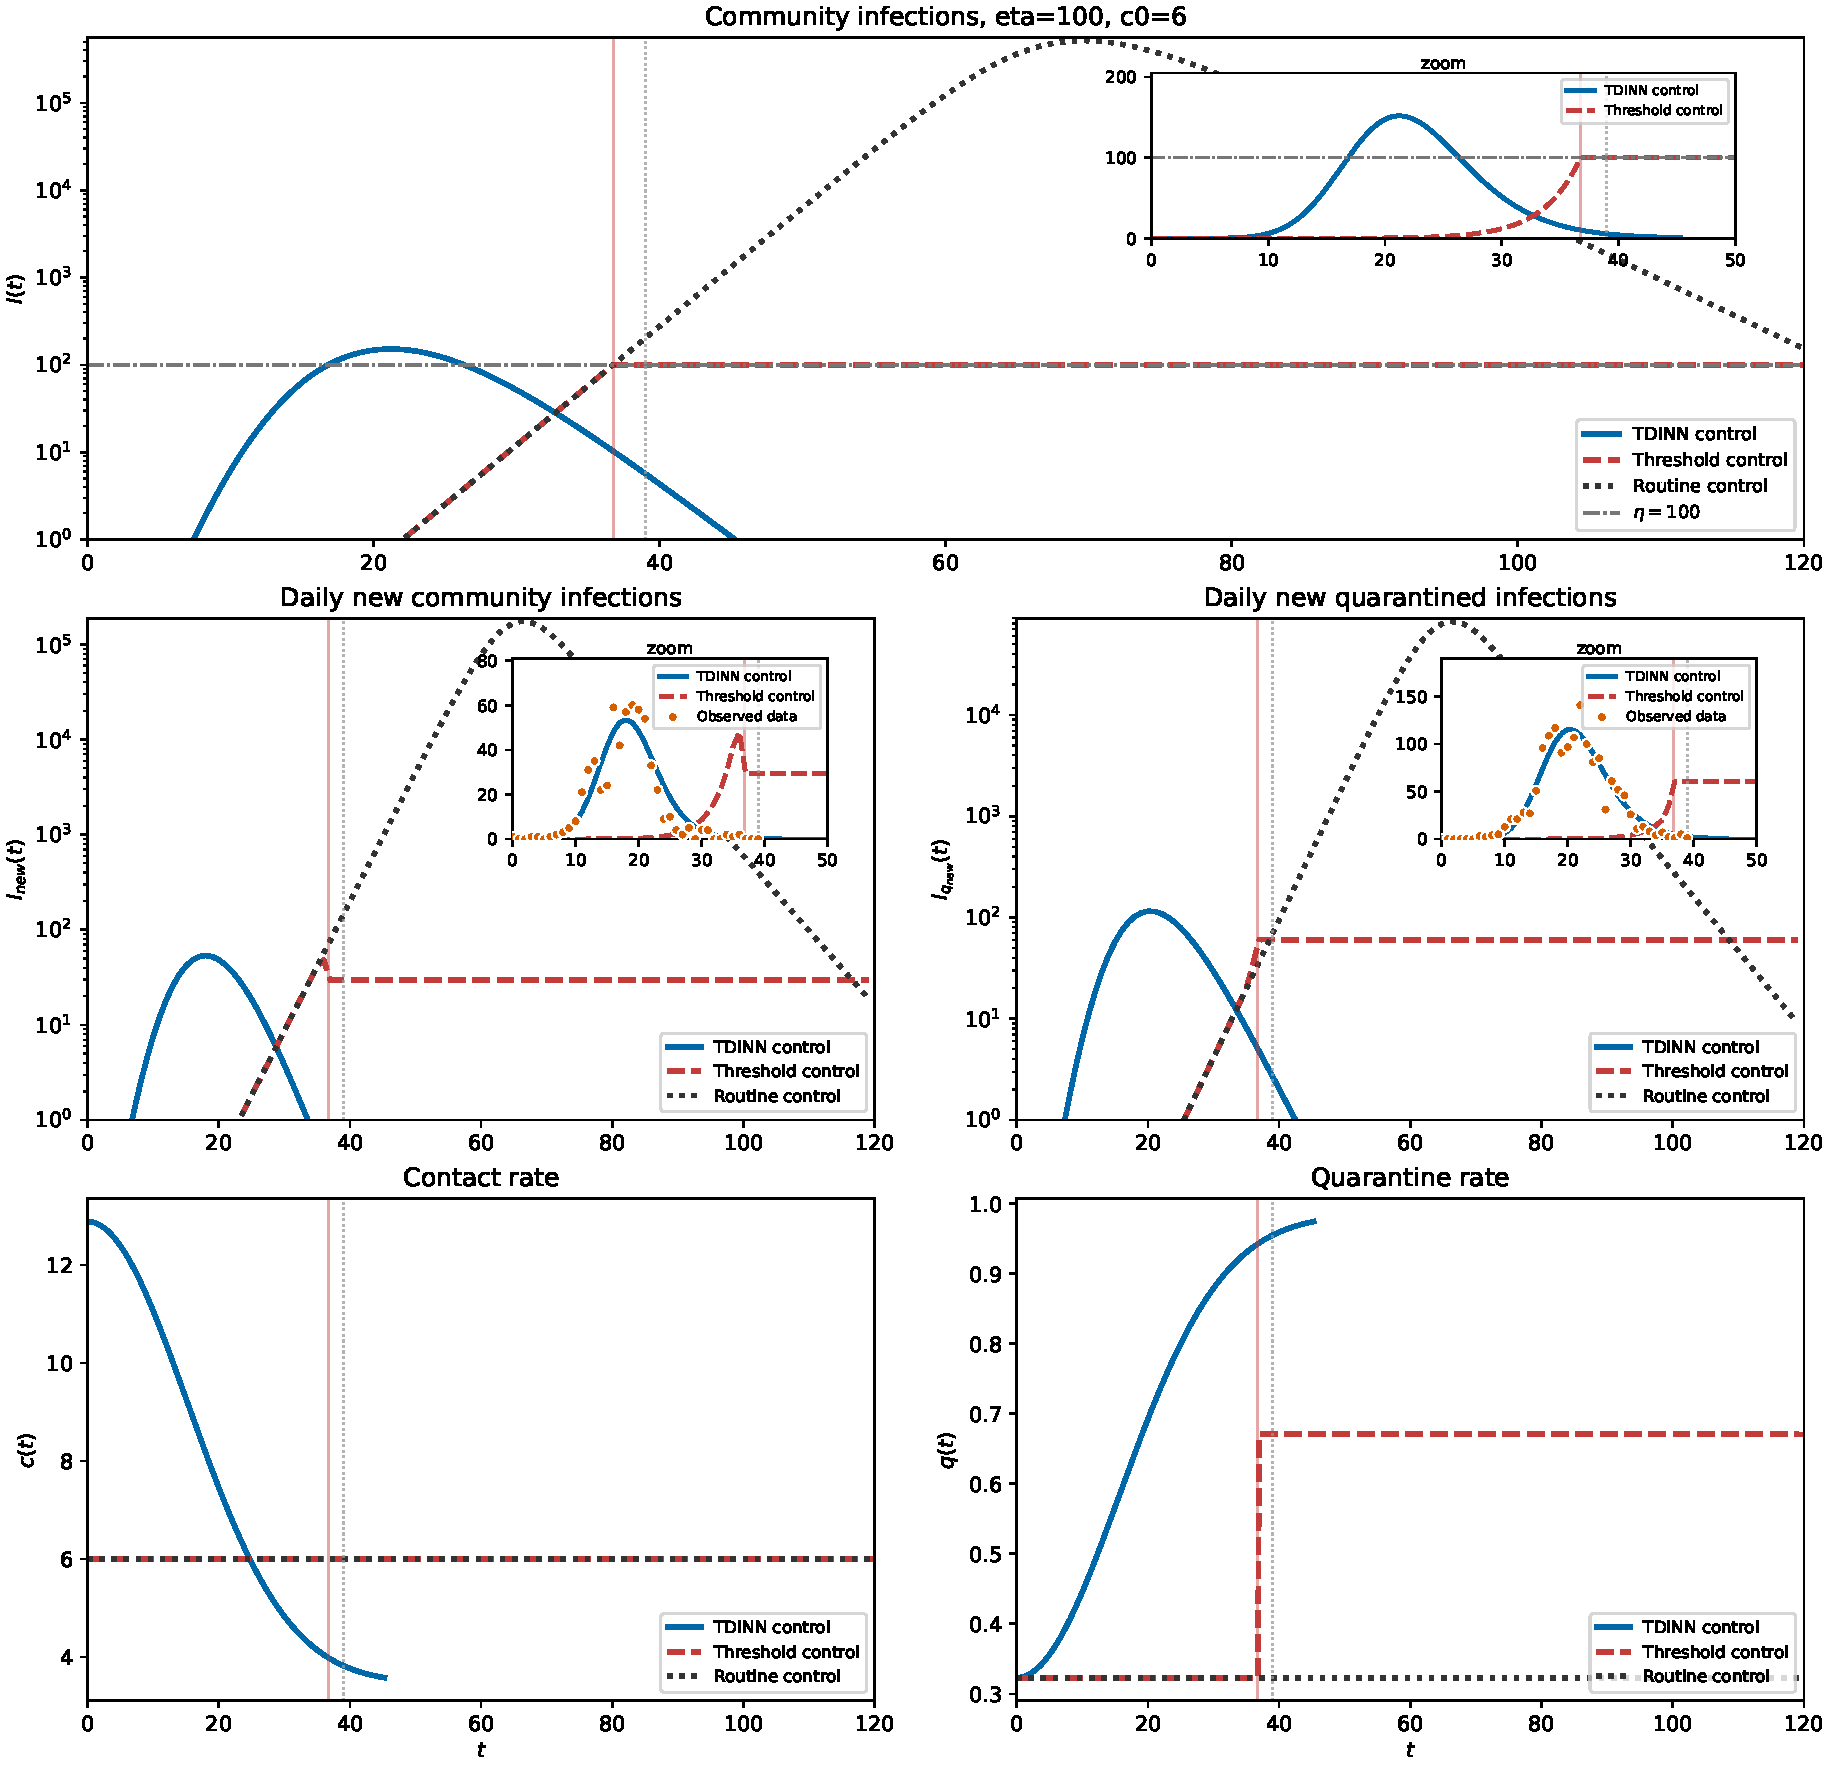
\includegraphics[width=0.95\textwidth,height=0.64\textheight,keepaspectratio]{panels_eta100_c0_6p0.pdf}
  \caption{$\eta=100,c_0=6$ 时的轨迹比较。TDINN控制为固定参照，情景一阈值控制和常规控制均使用 $c_0=6$。}
  \label{fig:c0-6-panel}
\end{figure}

\begin{figure}[htbp]
  \centering
  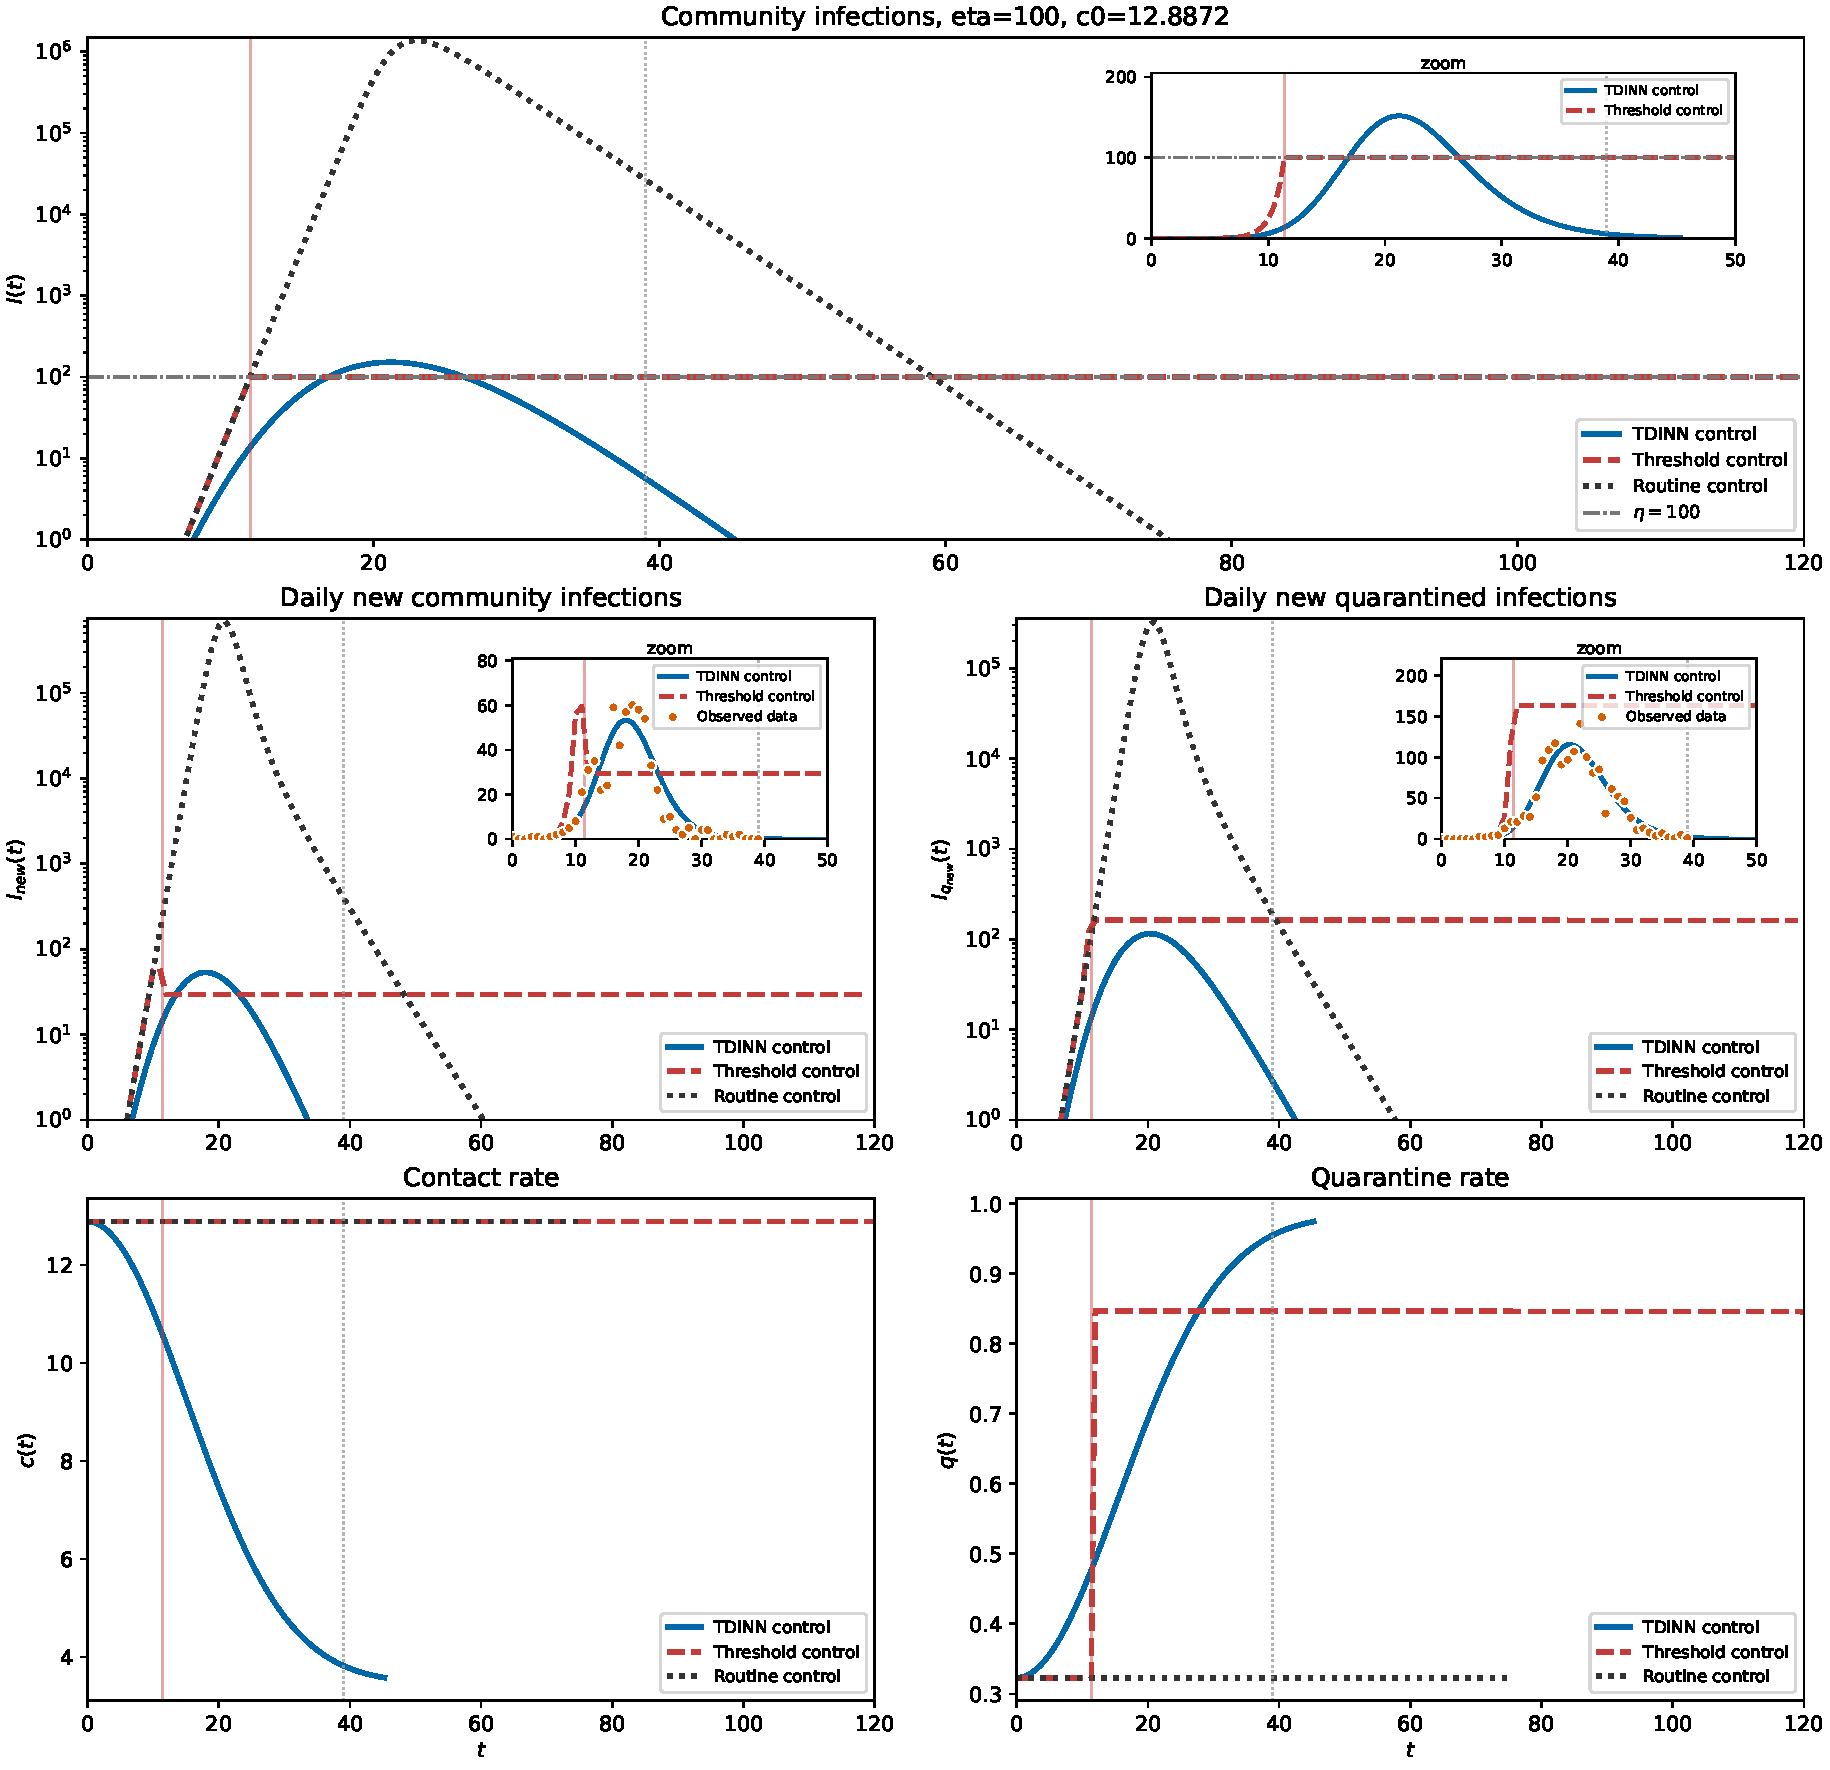
\includegraphics[width=0.95\textwidth,height=0.64\textheight,keepaspectratio]{panels_eta100_c0_12p8872.pdf}
  \caption{$\eta=100,c_0=12.8872$ 时的轨迹比较。}
  \label{fig:c0-base-panel}
\end{figure}

\section{较高接触率补充计算}

主分析中 $c_0=13$ 近似对应 TDINN 拟合初始接触率 $12.8872$ 的圆整上界。为了观察更高接触水平下公式的行为，额外计算
\begin{equation}
  c_0\in\{14,18,20\},
  \qquad
  \eta\in\{100,1300,26326\}.
\end{equation}
这组计算不改变主敏感性区间，只用于观察较高接触率下情景一控制律的数值边界。

\begin{table}[H]
  \centering
  \caption{较高接触率补充计算的可行性和时间指标。}
  \label{tab:high-c0}
  {\small
  \renewcommand{\arraystretch}{0.92}
  \resizebox{0.92\textwidth}{!}{
  \begin{tabular}{ccccccc}
    \toprule
    $c_0$ & $\eta$ & $t_1$ & $\Delta t$ & $t_{\rm end}$ & $q_{\max}$ & status\\
    \midrule
    14 & 100 & 10.24 & 21622.80 & 22797.67 & 0.8592 & ok\\
    14 & 1300 & 12.52 & 1662.90 & 2143.22 & 0.8591 & ok\\
    14 & 26326 & 15.20 & 81.70 & 247.24 & 0.8577 & ok\\
    18 & 100 & 7.52 & 18873.29 & 19908.54 & 0.8905 & ok\\
    18 & 1300 & 9.20 & 1451.51 & 1874.26 & 0.8904 & ok\\
    18 & 26326 & 11.17 & 71.38 & 216.70 & 0.8894 & ok\\
    20 & 100 & 6.64 & 17746.63 & 18728.53 & 0.9014 & ok\\
    20 & 1300 & 8.12 & 1364.88 & 1765.76 & 0.9014 & ok\\
    20 & 26326 & 9.86 & 67.14 & 204.96 & 0.9005 & ok\\
    \bottomrule
  \end{tabular}}}
\end{table}

\begin{figure}[htbp]
  \centering
  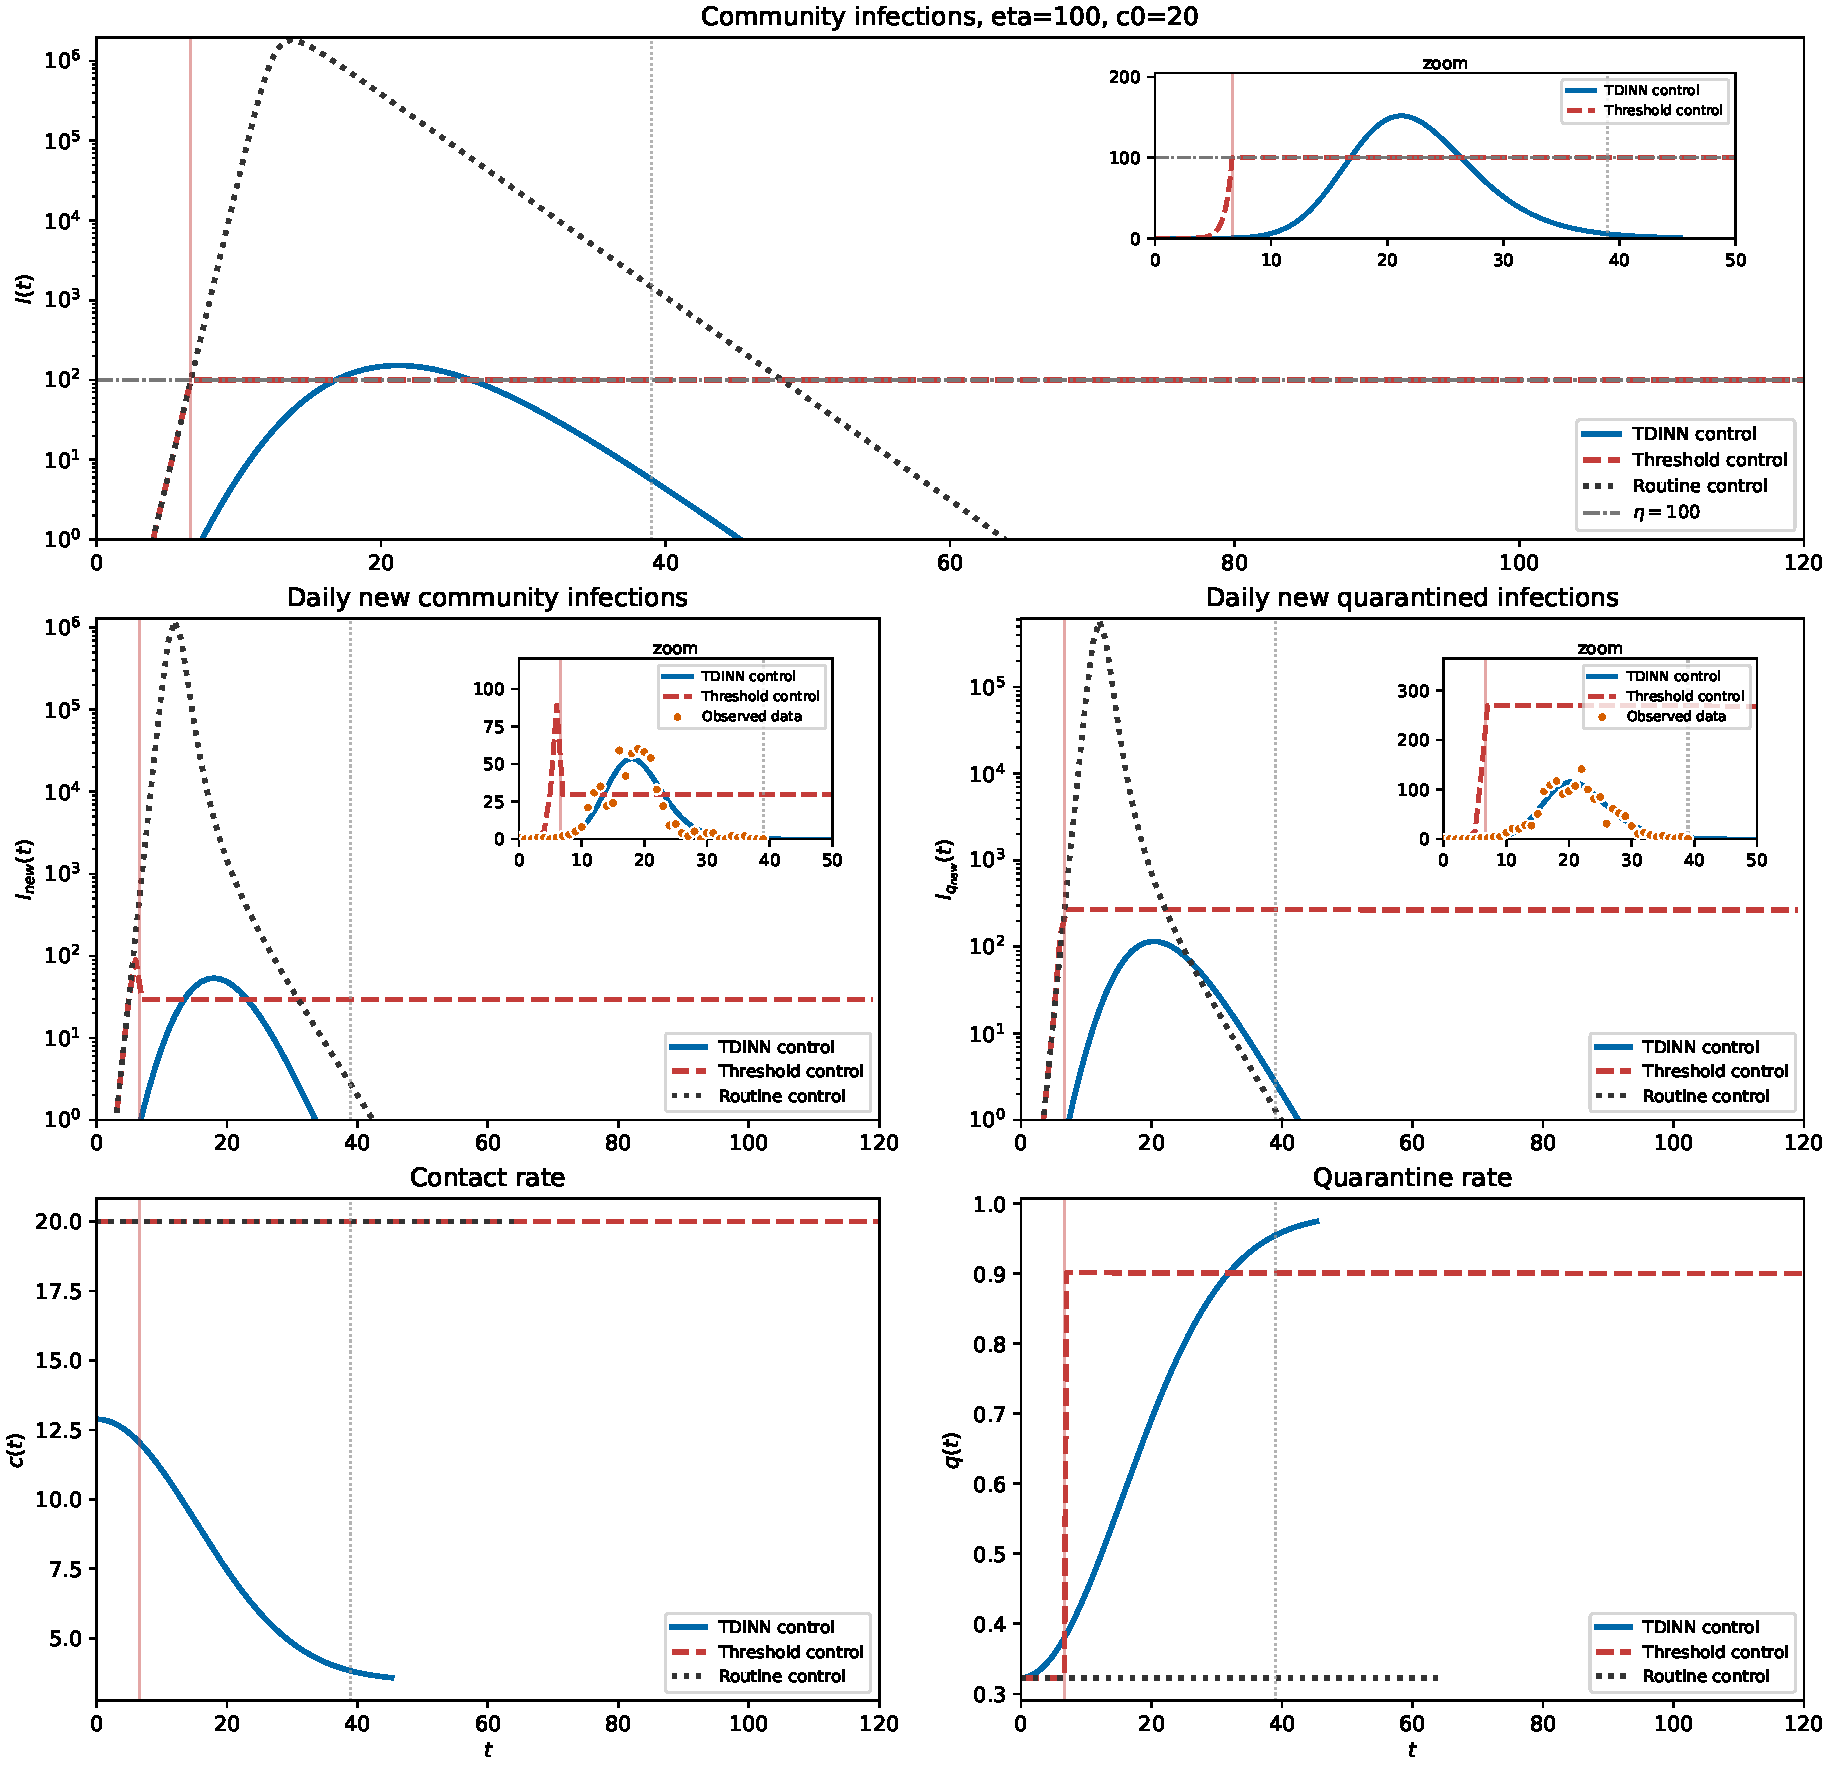
\includegraphics[width=0.95\textwidth,height=0.64\textheight,keepaspectratio]{stress_panels_eta100_c0_20.pdf}
  \caption{$\eta=100,c_0=20$ 的较高接触率补充计算。TDINN控制为固定参照，情景一阈值控制和常规控制均使用 $c_0=20$。}
  \label{fig:high-c0-panel}
\end{figure}

这些结果显示，提高 $c_0$ 可以缩短平台期，但不能消除低阈值带来的长期控制时间尺度。例如 $\eta=100,c_0=20$ 时，$\Delta t$ 仍约为 $17746.63$ 天。另一方面，$c_0$ 增大会提高所需隔离率，$c_0=20$ 时 $q_{\max}$ 约为 0.90。这个数值仍在 $[0,1]$ 内，但已经接近较高隔离强度。

\section{阶段性讨论}

在当前西安参数设定下，单阈值控制的主要矛盾不是公式能否构造，而是阈值选择带来的时间尺度。低阈值可以把社区感染者峰值限制在较小水平，但因为平台期满足 $I(t)=\eta$，易感者消耗速度变慢，$\Delta t$ 和 $t_{\rm end}$ 会显著增加。这个现象来自式 \eqref{eq:t2} 中的 $1/\eta$ 因子。

$c_0$ 的作用不同。较大的 $c_0$ 使常规阶段更快到达阈值，因此 $t_1$ 提前；平台期中 $S(t)$ 消耗也更快，因此 $\Delta t$ 缩短。但是，较大的 $c_0$ 同时要求更高的隔离率 $q_c(t)$。因此，$c_0$ 主要调节启动速度和隔离强度，而 $\eta$ 主要决定平台期的长短。

所有当前扫描点的状态均为 \texttt{ok}，说明在这些参数下 $q_c(t)$ 没有超出 $[0,1]$，数值轨迹也能保持 $I(t)=\eta$。这只是数学可行性。若要讨论现实可行性，还需要把 $q_c(t)$ 的实施含义、长期维持成本、医疗容量换算和观测误差放入同一个框架中。

\begin{remark}
  本笔记只整理单阈值控制的图谱结果。双阈值、预警阈值或同时调节 $c(t)$ 与 $q(t)$ 的控制方案属于后续问题，不在这里展开。
\end{remark}

\end{document}


情景一实现动态清零所需时间$t_{end}$:

\[
I(t)
=
-\frac{\beta_2^0}{\beta_1^0} S(t)
-
\rho_1 \ln S(t)
+
C_0
\qquad
t \in [t_2,+\infty)
\]

由$I(t_{end})=1$和$I'(t_{end})<0$得到
\[
1
+
\frac{\beta_2^0}{\beta_1^0} S(t_{end})
-
\rho_1 \ln(S(t_{end}))
=
C_0 .
\]

且\(S(t_{end}) < \frac{\gamma}{\beta_2^0}.\)使用 Lambert \(W\) 函数，求解 \(S(t_{end})\) 的方程，我们得到
\[
S(t_{end})
=
-\frac{\beta_1^0 \rho_1}{\beta_2^0}
\,
\operatorname{LambertW}_0
\left(
-\frac{\beta_2^0}{\beta_1^0 \rho_1}
\exp\left(
\frac{1-C_0}{\rho_1}
\right)
\right).
\]

现有
\[
S'(t)
=
S\left[
\beta_2^0 S
-
\beta_1^0 \rho_1 \ln(S)
-
\beta_1^0 C_0
\right],
\qquad
t \in [t_2,+\infty).
\]

从时间 \(t_2\) 积分到 \(T_{\mathrm{end}}\)，有
\[
\int_{S(t_2)}^{S(T_{\mathrm{end}})}
\frac{1}
{
S\left[
\beta_2^0 S
-
\beta_1^0 \rho_1 \ln(S)
-
\beta_1^0 C_0
\right]
}
\, dS
=
\int_{t_2}^{T_{\mathrm{end}}} dt .
\]

因此
\[
T_{\mathrm{end}}
=
t_2
+
\int_{S(t_2)}^{S(T_{\mathrm{end}})}
\frac{1}
{
S\left[
\beta_2^0 S
-
\beta_1^0 \rho_1 \ln(S)
-
\beta_1^0 C_0
\right]
}
\, dS .
\]
